\documentclass[a4paper]{article}

%%%%%%%%%%%%%%%%%%%%%%%%%%%%%%%%%%%%%%%%%%%%%%%%%%%%%%%%%%%%%%%%%%%%%%
% Imports.
%%%%%%%%%%%%%%%%%%%%%%%%%%%%%%%%%%%%%%%%%%%%%%%%%%%%%%%%%%%%%%%%%%%%%%

\usepackage{amsmath,amssymb,amsfonts}  % Typical maths resource packages
\usepackage{graphics}                  % Packages to allow inclusion of graphics
\DeclareGraphicsExtensions{.pdf,.png}
\usepackage{epstopdf}				   % Package to avoid errors on .eps to pdf conversions

\usepackage{fancyhdr}				   % Redesign the header and footer
\pagestyle{fancy}
\fancyfoot{}
\fancyhead{}
\fancyhead[OR]{\thepage}
\fancyhead[EL]{\thepage}


%\usepackage[T1]{fontenc}			   % Vectoriel fonts
\usepackage[french]{babel}			   % For french quotes
\usepackage{xcolor, url}			   % For links' colour

\usepackage{color}                     % For creating coloured text and background
\usepackage{hyperref}                  
\usepackage{textcomp}

\usepackage{xcolor}

% Listings settings.
\usepackage{courier}
\usepackage{caption}
\DeclareCaptionFont{white}{\color{white}}
\DeclareCaptionFormat{listing}{\colorbox[cmyk]{0.95, 0.95, 0.95,0.01}{\parbox{\textwidth}{\hspace{15pt}#1#2#3}}}
\captionsetup[lstlisting]{format=listing,labelfont=white,textfont=white, singlelinecheck=false, margin=0pt}

\usepackage{float}
\usepackage[hyperref,framed]{ntheorem} % For creating nice definition boxes
\usepackage[all]{hypcap}
\usepackage{framed}
\usepackage{pstricks}
\usepackage{listings}                  % For code listings
\usepackage{makeidx}                   % For generating index
\usepackage{enumitem}				   % http://ctan.org/pkg/enumitem
\usepackage[nohyperlinks]{acronym}
\usepackage{Msc}

\RequirePackage[left=2.4cm,right=2.4cm,bottom=2cm]{geometry} % Redefine the page margins
%\usepackage[hmargin=2.4cm]{geometry}

\renewcommand{\labelitemi}{$\bullet$}

\renewcommand\lstlistingname{Listing}
\renewcommand\lstlistlistingname{List of listings}

%%%%%%%%%%%%%%%%%%%%%%%%%%%%%%%%%%%%%%%%%%%%%%%%%%%%%%%%%%%%%%%%%%%%%%
%\parindent 1cm
%\parskip 0.2cm
%\topmargin 0cm
%\bottommargin 0cm
%\rightmargin 0cm
%\leftmargin 0cm
%\oddsidemargin 1cm
%\evensidemargin 0.5cm
%\textwidth 15cm
%\textheight 21cm
%\makeindex

%%%%%%%%%%%%%%%%%%%%%%%%%%%%%%%%%%%%%%%%%%%%%%%%%%%%%%%%%%%%%%%%%%%%%%
%\renewcommand{\familydefault}{\sfdefault}

%%%%%%%%%%%%%%%%%%%%%%%%%%%%%%%%%%%%%%%%%%%%%%%%%%%%%%%%%%%%%%%%%%%%%%
% where are figures
\graphicspath{
  {./}
  {figures/}
  }

%%%%%%%%%%%%%%%%%%%%%%%%%%%%%%%%%%%%%%%%%%%%%%%%%%%%%%%%%%%%%%%%%%%%%%
%hyperref settings
\hypersetup{pdfauthor=Thomas Rouvinez, 
            pdftitle=HL7 Exchange Module, 
            pdfsubject=YourBookSubjectHere,
            colorlinks=true,
            linkcolor=black}

%%%%%%%%%%%%%%%%%%%%%%%%%%%%%%%%%%%%%%%%%%%%%%%%%%%%%%%%%%%%%%%%%%%%%%
% redefine some colors
\definecolor{shadethmcolor}{rgb}{0.9412,.9412,1.0000} % 
\definecolor{shaderulecolor}{rgb}{0.1529,0.2510,0.5451} % RoyalBlue 
\definecolor{lightergray}{gray}{0.95}
\definecolor{palegreen}{rgb}{0.7148,0.9219,0.6797} %pale green

%%%%%%%%%%%%%%%%%%%%%%%%%%%%%%%%%%%%%%%%%%%%%%%%%%%%%%%%%%%%%%%%%%%%%%
% define the theorem environments
% 1. definition
\theoremstyle{break}
\shadecolor{shadethmcolor}
\def\theoremframecommand{% 
\psframebox[fillstyle=solid,fillcolor=shadethmcolor,linecolor=shaderulecolor]} 
\newshadedtheorem{definition}{Definition}[section]
% 2. remark
\theoremstyle{plain} 
\theoremheaderfont{\normalfont\footnotesize\bfseries} 
\theorembodyfont{\normalfont\footnotesize} 
\theoremsymbol{\ensuremath{\clubsuit}} 
\theoremseparator{.}
\theoremindent1cm 
\theoremprework{\smallskip} 
\theorempostwork{\smallskip} 
\newtheorem*{remark}{$\rightarrow$ Remark}
% 3. seobs (software engineering observation)
\theoremstyle{plain} 
\theoremheaderfont{\normalfont\bfseries}
\theorembodyfont{\normalfont\normalsize}  
\theoremsymbol{\ensuremath{\clubsuit}} 
\theoremindent0cm 
\theoremseparator{.} 
\theoremprework{\bigskip\hrule} 
\theorempostwork{\hrule\bigskip} 
\newtheorem{seobs}{Software Engineering Observation}[section]
% 4. program output
\theoremstyle{nonumberplain} 
\theoremindent0.5cm 
\theorembodyfont{\ttfamily\small}
\theoremindent0cm 
\theoremseparator{} 
\theoremprework{\bigskip\verb}
\theorempostwork{\bigskip} 
\shadecolor{shadethmcolor}
\def\theoremframecommand{% 
\psframebox[fillstyle=solid,fillcolor=palegreen,linecolor=palegreen]} 
\newshadedtheorem{programoutput}{}

%%%%%%%%%%%%%%%%%%%%%%%%%%%%%%%%%%%%%%%%%%%%%%%%%%%%%%%%%%%%%%%%%%%%%%
% settings for the listings

\definecolor{green}{RGB}{0,180,10}
\definecolor{dkgreen}{rgb}{0,0.6,0}
\definecolor{gray}{rgb}{0.5,0.5,0.5}
\definecolor{mauve}{rgb}{0.58,0,0.82}

\lstset{
		language=Java,                % the language of the code
  		basicstyle=\footnotesize\ttfamily, % Standardschrift
        numbers=left,               % Ort der Zeilennummern
        numberstyle=\tiny,          % Stil der Zeilennummern
        stepnumber=1,               % Abstand zwischen den Zeilennummern
        numbersep=8pt,              % Abstand der Nummern zum Text
        tabsize=2,                  % Groesse von Tabs
        extendedchars=true,         %
        breaklines=true,            % Zeilen werden Umgebrochen
        commentstyle=\color{dkgreen},
        keywordstyle=\color{mauve},
    	   frame=b,         
        stringstyle=\color{blue}\ttfamily, % Farbe der String
        showspaces=false,           % Leerzeichen anzeigen ?
        showtabs=false,             % Tabs anzeigen ?
        xleftmargin=17pt,
        framexleftmargin=17pt,
        framexrightmargin=5pt,
        framexbottommargin=4pt,
        %backgroundcolor=\color{lightgray},
        showstringspaces=false      % Leerzeichen in Strings anzeigen ?     
 }

\begin{document}
\pagenumbering{roman}

%%%%%%%%%%%%%%%%%%%%%%%%%%%%%%%%%%%%%%%%%%%%%%%%%%%%%%%%%%%%%%%%%%%%%%
% Custom commands.
%%%%%%%%%%%%%%%%%%%%%%%%%%%%%%%%%%%%%%%%%%%%%%%%%%%%%%%%%%%%%%%%%%%%%%

\newenvironment{listCustom}{
 \begin{list}{{$\bullet$}}{		% type of item representation
  \setlength{\partopsep}{0pt}
  \setlength{\parskip}{0pt}
  \setlength{\parsep}{0pt}
  \setlength{\topsep}{5mm}
  \setlength{\itemsep}{1mm}		% space between items
  \setlength{\labelsep}{0.25cm} % bullet to text distance
  \setlength{\leftmargin}{2cm}  % reset margin
 }
}{
 \end{list}
}

{\setlength{\leftmargini}{2cm} 
\newenvironment{listCustomNumber}{
 \begin{enumerate}{		% type of item representation
  \setlength{\leftmargin}{2cm}  % reset margin
 }
}{
 \end{enumerate}
}

\newcommand*{\xml}[1]{\texttt{<#1>}}

\newcommand*{\webquote}[1]{\textsf{\og #1 \fg{}}}
\renewcommand*\abstractname{Abstract}
\renewcommand*\contentsname{Table of Contents}
	
%%%%%%%%%%%%%%%%%%%%%%%%%%%%%%%%%%%%%%%%%%%%%%%%%%%%%%%%%%%%%%%%%%%%%%
% Title page.
%%%%%%%%%%%%%%%%%%%%%%%%%%%%%%%%%%%%%%%%%%%%%%%%%%%%%%%%%%%%%%%%%%%%%%

\title{BitTorrent distributed generation of rainbow tables}
\course{Advanced Networking and Future Internet}

\author{Arnaud Durand, Mikael Gasparian, Thomas Rouvinez}
\professor{Prof. Dr. Torsten Braun, Dr. Tuan Anh Trinh, Dr. I. Aad}
\date{06 January, 2014}


\rrno{}
\maketitle

\pagebreak


%%%%%%%%%%%%%%%%%%%%%%%%%%%%%%%%%%%%%%%%%%%%%%%%%%%%%%%%%%%%%%%%%%%%%%
% Content Table.
%%%%%%%%%%%%%%%%%%%%%%%%%%%%%%%%%%%%%%%%%%%%%%%%%%%%%%%%%%%%%%%%%%%%%%
	
\tableofcontents

\pagebreak

\pagenumbering{arabic}

%%%%%%%%%%%%%%%%%%%%%%%%%%%%%%%%%%%%%%%%%%%%%%%%%%%%%%%%%%%%%%%%%%%%%%
% Document's body.
%%%%%%%%%%%%%%%%%%%%%%%%%%%%%%%%%%%%%%%%%%%%%%%%%%%%%%%%%%%%%%%%%%%%%%

\begin{abstract}
In this paper, we discuss the possibility to use the BitTorrent protocol as a way to distribute a workload to be processed by multiple nodes. We create our own implementation and use the rainbow tables generation process as a test application. We present our results, the torrent library we chose to enhance as well as the modifications we operated on it.
\end{abstract}
\vspace{2mm}

\section{Introduction}

Moore's law applies to our current state of technologies with periodic improvements of the computing power available in a single processing unit. Along side this evolution goes the always growing need for more processing power as scientists can count on large improvements on the hardware level within a couple of years. Since we expect such an improvement to happen, we tend to design algorithms with higher accuracy and number of input parameters to process. Unfortunately a single processing unit is still far from providing enough processing power to solve such problems, whereas distributing the work on many computers can.\\

Following this spirit we can consider distributed computing as a solution that comes with a price : the efficiency / performances ratio. For a workload to be efficiently processed, we need a work that is splitable in sub-tasks, each computable independently (no precedence of computation issues). Another liability remains in the way to gather back all computations. This is where the BitTorrent protocol can be helpful : a torrent file is split in a given number of files, each split in a given number of pieces. Each piece can already be downloaded or not.Provided that the two conditions explained above for distributed computing are granted, we could transform a torrent that downloads the rarest pieces into a torrent that generates the rarest pieces.\\

BitTorrent is often considered in distribued computing, but only as a mean to store large amounts of data. Our goal for this project is to actively use the BitTorrent protocol to transform each servent node into a computing node that would make the pieces it computed available to other nodes for download. An application requiring a significant amount of processing power and that can easily be split is rainbow tables generation, which we will use as a proof of concept application.\\

In this report, we will explore what are rainbow tables and how they can be generated on multiple machines. We will also present the modifications we operated on the existing BitTorrent protocol to allow us to piggyback computed data from the nodes. Finally, we will present the results of our implementation.

\section{Tools and libraries}

We chose to use Java as main programming language for this project since it is adequate to develop a prototype quickly. Moreover there are already many existing libraries that handle the generic BitTorrent protocol written in Java.\\

To develop this project, we used the following programs :

\begin{listCustom}
	\item Eclipse IDE
	\item RTGen (RainbowCrack\footnote{Source : \url{http://www.project-rainbowcrack.com/}})
	\item Bencode editor v0710u\footnote{Source : \url{https://sites.google.com/site/ultimasites/bencode-editor}}
	\item GitHub
	\item LaTeX
\end{listCustom}

We chose to start with "\textbf{Turn's BitTorrent}"\footnote{Source : \url{http://mpetazzoni.github.io/ttorrent}} library because it is an open-source project (Apache License 2.0) and is easy-to-embed in any program. Ttorrent has also a very clean code and provides a tracker / client source code already.

\section{Distributed computation with BitTorrent}

The BitTorrent protocol is used to download files from a network made of nodes which are both servers and clients. Servers because they have a list of peers who share the same files and clients because they are looking to download these same files. The initial information is contained in the .torrent file (tracker URI, files, piece size, etc). Let us denote by \textbf{RTTorrent} a torrent file that holds specific additional information for rainbow tables generation.
\vspace{2mm}

\begin{figure}[H]
  \centering
    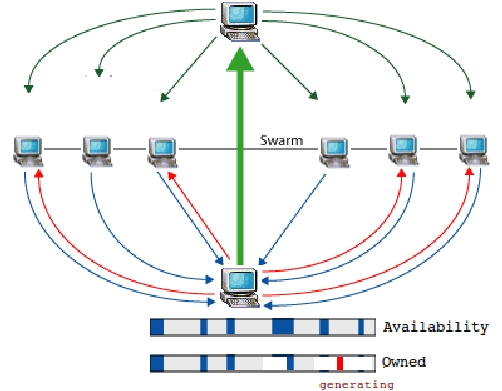
\includegraphics[scale=0.5]{schema.jpg}
    \caption{RTTorrent pinciple}
    \label{principle}
\end{figure}
\vspace{2mm}

Each time a new torrent is launched, the client will map its neighbors thanks to the tracker and compute the availability of each piece of the files to download. The rarest piece is selected and downloaded, then marked as "Have" to let other know this piece is available from our client now. If no peer has a piece, we have to wait until a new peer connects and has the piece we are looking for. With RTTorrent, the difference is that if a piece is not available we can generate it by launching an instance of RTGen on the node (cf. figure \ref{principle}). Once the piece is computed, the peers can download it (no need to generate it).

\section{Modifications to Turn's library}

This section describes all the modifications we had to operate to tranform Turn's library into a rainbow tables torrent library. Note that we have specified in the code which part we have altered to enable support for the new features.

\subsection{Torrent file specification}

To enable a torrent to carry the required information to compute hash tables, we had to modify the specification 
of the .torrent file. We added the following fields to the already existing BitTorrent fields :

\begin{center}
\begin{tabular}{|l|l|}
\hline 
\textbf{Field} & \textbf{Description} \\ 
\hline 
chainLength & The rainbow chain length. Longer chains store more plaintexts (longer to generate)\\ 
\hline 
plaintextLenMin & These two parameters limit the plaintext length range of the rainbow table\\ 
\hline 
plaintextLenMax & These two parameters limit the plaintext length range of the rainbow table\\ 
\hline 
pieceLength & The number of bytes in each piece\\ 
\hline 
charset & The charset includes all possible characters for the plaintext\\ 
\hline 
hashAlgorithm & Rainbow table is hash algorithm specific\\
\hline 
\end{tabular} 
\end{center}
\vspace{3mm}

To enable the torrent to recognize these fields that are not specified in the original BitTorrent protocol, we had to modify the parsing of the .torrent files. In addition to the previously mentioned fields, we added a "table index" field in each file that the torrent is supposed to download. This parameter selects the reduction function. Rainbow table with different table index parameter uses different reduction function.

\subsection{Rainbow tables generation}

Each time a piece is unavailable for download among all the connected peers, the RTTorrent starts generating one. We had to implement a new thread for the generation aside the regular download threads. If a piece is missing, we randomly select one of the remaining pieces (see chapter 4.3) to download and start generating the related rainbow table.\\

To generate a piece, we use the RainbowCrack Project RTGen that we can call from a dedicated thread on any client node. The piece to compute is selected at random from the array of unavailable pieces. Then we provide RTGen with the information on the hash algorithm, charset, plain text minimum and maximum length and the chain length, all previously stored in the .torrent file.\\

Once the required tables are generated, they are stored in the data byte array of a new piece, which in turn is recorded in the general files of the torrent. Once the piece is secured we can treat it as a completed download by tagging that piece as "complete" and by sending to all connected peers a "Have" message so they are aware that this piece is available for download.

\subsection{Piece selection and validation}
In a regular Torrent, the selection of the next piece to download is made upon a set of rarest pieces among the peers connected to a given node. Each time a piece is downloaded and validated, this piece is removed from the rarest list and the next one starts downloading. As we don't have the problem of having nonexistent pieces with RTTorrent (since we can generate them), we have to find new strategies to select the next piece to generate :\vspace{2mm}

\begin{enumerate}
	\item Choose first piece from k pieces where k is unavailable. This translates into picking the first missing piece in the vector of missing pieces. This means that almost every peer will select the same piece, thus yielding a nearly  100\% collision rate.
	\item Choose random piece from k pieces. When not optimal, it drastically reduced the collision rate at the beginning of the process, but the more complete the RTTorrent, the more collisions will happen.
	\item Choose a piece k based on peers agreement using communication. This synchronizes the generation by keeping an internal tracking of the currently generated pieces. This is the most efficient solution, but it induces more traffic and validations for each node.
	\item Choose piece from k based on neighbors peer IDs. This achieves relatively the same as strategy 3, but no communication is required because we compute wich peer ID compared to our own ID computes which piece. There are no additional communications induced.
\end{enumerate}
\vspace{2mm}

This project being a proof of concept, we chose strategy number 2 for its ease of implementation compared to its performances. The best solution would be strategy number 4 though for optimal performances and robustness.\\

Compared to a common Torrent, the RTTorrent cannot operate a regular validation on the chunks downloaded for two reasons : first the pieces that do not exist are generated, which means we do not know their hash to validate them. Second validating received chunks means recomputing them, which defeats the purpose of distributing the workload. Therefore we set valid field of each piece downloaded to true.

\subsection{Torrent client}

With all the previously mentioned modifications brought to the code, the regular torrent client could not work anymore without adaptations :

\begin{figure}[H]
  \centering
    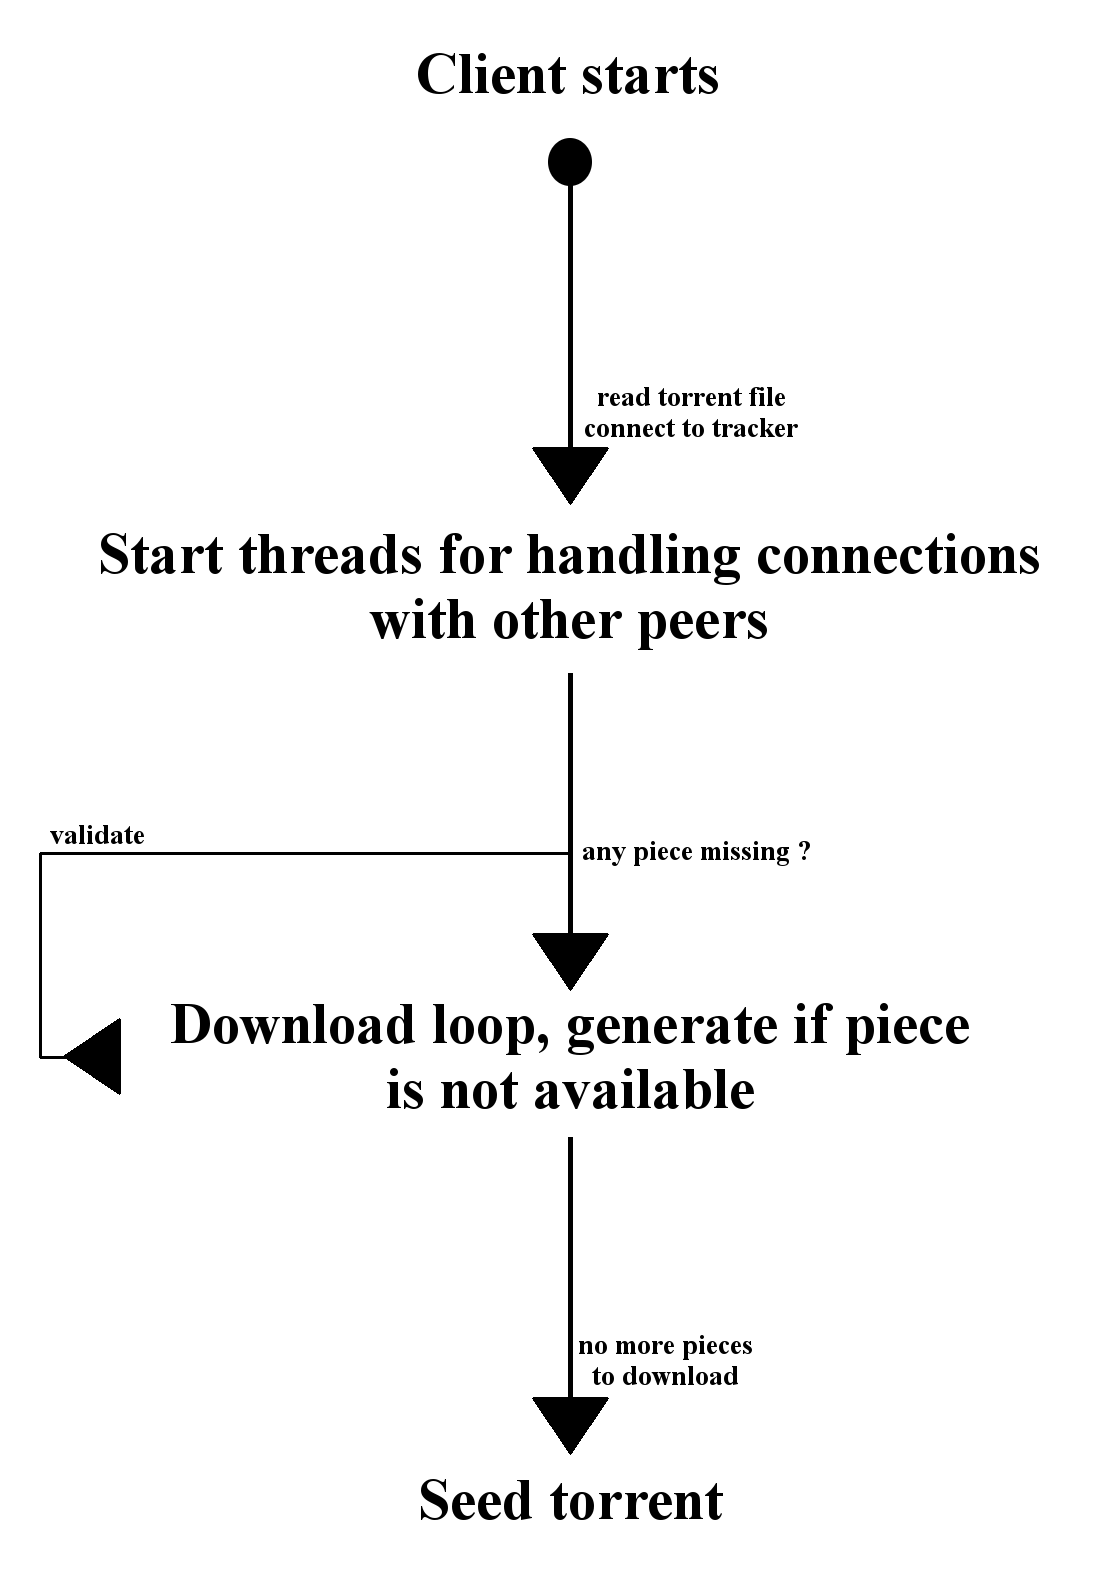
\includegraphics[scale=0.2]{works.png}
    \caption{Client workflow}
    \label{works}
\end{figure}
\vspace{2mm}

In the original Turn's library, the client starts by initializing a "ShareTorrent" object from a torrent meta-info source (either a file or a byte array, see com.turn.ttorrent.SharedTorrent). Then, it instantiates the Client object with this SharedTorrent and downloads the torrent and continues seeding for the given amount of time after the download completes.\\

For this project we had to modify the download process so that instead of waiting for a piece that is unavailable, we start generating it via a callable execution. \\

TO COMPLETE

\section{Experiments and results}

To test our library, we created a custom torrent containing two file, each made of 32 pieces. Each piece weighs one MB. We chose to use small pieces with a small charset length for the purpose of demonstration : with such parameters, we can generate a new piece roughly every 15 seconds.\\

No tit-for-that

\section{Improvements}

Being a proof of concept, this project's main focus is to provide a working RTTorrent library on which various improvements such as the following ones can be made :\\

\begin{description}
	\item [Interrupt exception : ] it may happen that a piece becomes available while we are generating it. This would occur if a given piece is not downloadable at time X so that the node starts generating it and finishes at time Z, but another node finishes to generate that same piece at time Y. To avoid such waste of processing power, we could implement an interrupt exception in case we receive a message "Have" from another peer on a piece we are currently generating.\\
	
	\item [Pause/resume state : ] Torrent networks often get peers connecting and disconnecting, not always in a gentle manner. Considering that generating a piece takes more time than downloading the generated piece, it would be better to be able to resume state on application reload.\\
	
	\item [Piece selection : ] as discussed in chapter 4.3, we are currently selecting randomly which will be the next piece to generate on a node. This strategy loses performances the closer we are to the end of the torrent's download. Strategy number 3 or 4 should be considered instead, depending on what are the needs for the final application.\\
	
	\item [Piece validation] : currently no verification can be operated since the time required to verify a piece is greater than the generation time of that same piece. A solution could be to download randomly pieces and re-generate them, then compare with the downloaded ones. Also some pieces could be asked from multiple different peers and compared, which spares the regeneration time waste. The each peer could tag a bad peer so others stop downloading from it.
\end{description}

\section{Conclusions}

Through this project we have proven that the BitTorrent protocol, given the right modifications, can accommodate distributed computations. Not only the workload is shared among the peers, but the original purpose of BitTorrent allows to share and store quickly the generated chunks together. It is also interesting to notice that a regular tracker can provide the bootstrap for RTTorrents and BitTorrents alike. Only the client is different since it has to be able to read the extra information contained in an RTTorrent and dedicate the generation process to an external software.\\

From a more conceptual perspective RTTorrents are an example of how distributed computations can be achieved via BitTorrent. Nevertheless all types of computations may not apply correctly to this process since we need a way to generate pieces resulting from the computation that have the same length.\\

Must trust the clients.

%%%%%%%%%%%%%%%%%%%%%%%%%%%%%%%%%%%%%%%%%%%%%%%%%%%%%%%%%%%%%%%%%%%%%%
% End of document.
%%%%%%%%%%%%%%%%%%%%%%%%%%%%%%%%%%%%%%%%%%%%%%%%%%%%%%%%%%%%%%%%%%%%%%

\end{document}